\newpage
\section{Results}
This section will give some simple examples of the previously described system to illustrate the implications of the barrier fluctuations coupled to the diffusive transport of Brownian particles.\\
It will also give a close examination of certain limits e.g. of very fast and very slow barrier fluctuations and compare these to simulation results. In addition, it will be evaluated if the solution for a step shaped barrier is a valid approximation for smooth potentials of similar shape depending on the timescale of the barrier fluctuations. \\
Finally it will show the effects that come from the transition of the barrier between two states due to independent variation of its HIGH $\rightarrow$ LOW and LOW $\rightarrow$ HIGH switching rates.
\subsection{A Two State Barrier with Symmetric Switching Rates}
The first example will be the most simple system possible consisting only of a two state barrier of hight $U_1 = 0$ and $U_2 \ne 0$ that is ether on or off. Also the barrier switching is symmetric i.e. the on $\rightarrow$ off and off $\rightarrow$ on rates are equal $\mathbb{W}_{12}=\mathbb{W}_{21}=W$ such that the potential of mean force acting on the Brownian particles is independent of the switching rate.
This allows for the detailed study of effects solely coming from the coupling of timescales between barrier fluctuations and diffusive transport without any other influence.
\subsection{Particle Density}
The first step for the investigation of the example is the calculation of the analytic solution for the density profiles of the Brownian particles. Therefore one first writes down the corresponding Fokker-Planck equation:
\begin{align}
    \frac{\partial \rho_1(r,t)}{\partial t} &= \vec \nabla \left[ D \vec \nabla \rho_1(r,t) \right] - W_{2,1}\rho_1(r,t) + W_{1,2}\rho_2(r,t) \nonumber \\
    \frac{\partial \rho_2(r,t)}{\partial t} &= \vec \nabla \left[\rho_2(r,t) \vec \nabla \frac{U_2(r)}{\gamma} + D \vec \nabla \rho_2(r,t) \right] - W_{1,2}\rho_2(r,t) + W_{2,1}\rho_1(r,t)
    \label{two_state_fpe}
\end{align}
Note that the particles in state $m=1$ move freely and are not subject to any potential barrier. 
Since the transition rates are symmetric $W_{1,2} = W_{2.1} = W$  the transition rate matrix has the form:
\begin{equation}
    \mathbb{W} = \left( \begin{array}{rr}
    W & -W \\
    -W & W 
\end{array} \right)
    \label{two_state_transition_matrix}
\end{equation}
With eigenvalues $\lambda_1 = 0$ and $\lambda_2 = -2W$. The steady state solution to the transition matrix is 
\begin{equation}
    \vect{\rho}^{(eq)}=\left(\frac{1}{2}, \frac{1}{2}\right)^{T}
    \label{rhoeq}
\end{equation}
which obviously satisfies the detailed balance property \eqref{detailed_balance}. \\
The diagonal form of equation \eqref{two_state_fpe} is now 
\begin{equation}
    \frac{\partial}{\partial t} \tilde{\vect{\rho}} = \left( \begin{array}{ll}
        D\vec{\nabla}^{2} & 0 \\
        0 & D\vec{\nabla}^{2} - 2W
    \end{array} \right) \tilde{\vect{\rho}}
    \label{fpmeq5}
\end{equation}
and the steady state solution in terms of eigenfunctions of $\mathbb{W}$ reads
\begin{align}
    \tilde{\rho}_1^{(k)} &= c_{1,1}^{(k)} + \frac{c_{1,2}^{(k)}}{r} \\
    \tilde{\rho}_2^{(k)} &= \frac{c_{2,1}^{(k)}}{r}{\rm exp}\left[-\frac{r}{r_d}\right]+ \frac{c_{2,2}^{(k)}}{r}{\rm exp}\left[\frac{r}{r_d}\right]
    \label{ind_sol_U2}
\end{align}
With the previously defined decay length $r_d$:
\begin{equation}
    r_d = \sqrt{\frac{d}{2W}}
    \label{rd_two_state}
\end{equation}
Once the coefficients $c^{(k)}_{i,j}$ are calculated from the boundary and fit conditions the density profiles can be plotted for several sets of parameters. If not stated differently, the parameters are given by the values in the following table. The choice of parameters is arbitrary now since the influence of each of them will be examined separately in later parts of this section.
\begin{equation}
    \begin{array}{r|l}
        Parameter & Value \\ \hline
        R_s & 1 \\
        a   & 6 \\
        b   & 11 \\
        U_2/K_B T & \mp 3 \\
    \end{array} \nonumber
    \label{Parameters}
\end{equation}
The first parameter that will be studied is the decay length $r_d$. The easiest way to get a first impression of its influence is to look at the density profiles. Therefore several examples for different parameter choices are given next.
For illustrative reasons the total particle density is normalized to $\rho_{tot}^{(eq)}=2$ for $r \rightarrow \infty$ in the following plots and the particle densities in the different states are depicted together with the mean particle density. \\
Since the state of the barrier can also be treated as a property of the Brownian particles as discussed in section \ref{Model_Description} it is convenient do so for the following discussion. The particles that are influenced by the barrier will hence be called \emph{active} whereas the particles that are not will be called \emph{inactive}. \\ In the following density plots the density of active particles is depicted in blue while the density of the inactive particles is depicted in red.

\begin{minipage}[t]{0.5 \textwidth}
    \begin{figure}[H]
        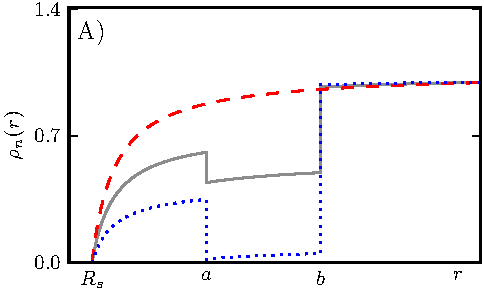
\includegraphics[width = 1 \textwidth]{plots/d1.pdf}
    \end{figure}
\end{minipage}
\begin{minipage}[t]{0.5 \textwidth}
    \begin{figure}[H]
        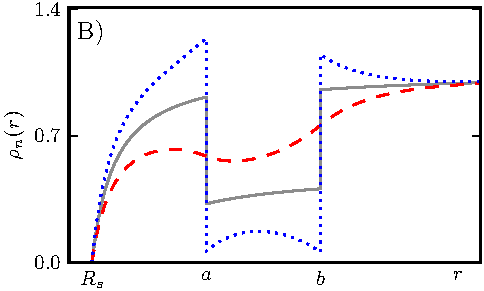
\includegraphics[width = 1 \textwidth]{plots/d2.pdf}
    \end{figure}
\end{minipage}
\begin{minipage}[t]{0.5 \textwidth}
    \begin{figure}[H]
        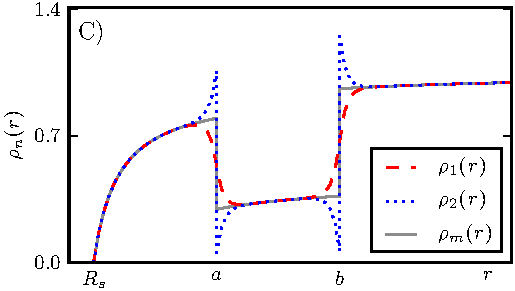
\includegraphics[width = 1 \textwidth]{plots/d3.pdf}
    \end{figure}
\end{minipage}\hspace{0.02\textwidth}\begin{minipage}[t]{0.48 \textwidth}
    \begin{figure}[H]
        \caption{Density profiles for repulsive fluctuating barrier. The densities of particles in state $m=1$ and state $m=2$ are depicted in dashed red, and dotted blue respectively. The decay length is given by A): $r_d = 250$, B): $r_d=2.5$ and C): $r_d=0.25$. \label{rep_symm_dens_profile}}
    \end{figure}
\end{minipage}


\begin{minipage}[t]{0.5 \textwidth}
    \begin{figure}[H]
        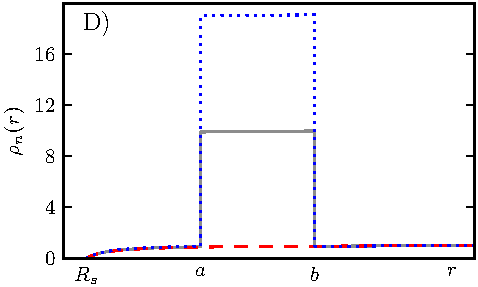
\includegraphics[width = 1 \textwidth]{plots/d4.pdf}
    \end{figure}
\end{minipage}
\begin{minipage}[t]{0.5 \textwidth}
    \begin{figure}[H]
        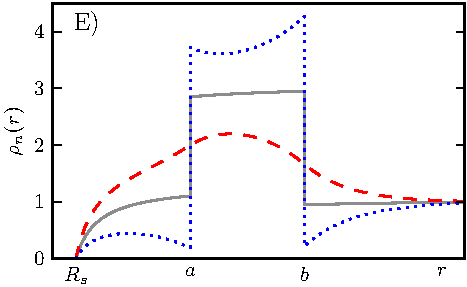
\includegraphics[width = 1 \textwidth]{plots/d5.pdf}
    \end{figure}
\end{minipage}
\begin{minipage}[t]{0.5 \textwidth}
    \begin{figure}[H]
        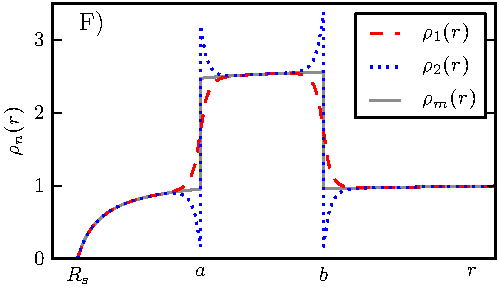
\includegraphics[width = 1 \textwidth]{plots/d6.pdf}
    \end{figure}
\end{minipage}\hspace{0.02\textwidth}\begin{minipage}[t]{0.48 \textwidth}
    \begin{figure}[H]
        \caption{Density profiles for attractive fluctuating barrier. The densities of particles in state $m=1$ and state $m=2$ are depicted in dashed red, and dotted blue respectively. The decay length is again given by A): $r_d = 250$, B): $r_d=2.5$ and C): $r_d=0.25$\label{att_symm_dens_profile}}
    \end{figure}
\end{minipage} 
\newpage
This case neatly illustrates the role of $r_d$ as the persistence length of the influence of the potential fluctuations. For distances $d_a = |r - a|$ and $d_b = |r - b|$ far from the jump discontinuities of the potential $d_a, d_b >> r_d$ the thermal motion of the Brownian particles dampens the influence of the potential barrier and the densities of active and inactive particles converge to the same value again.\\
So if $r_d$ is much larger as the overall spacing of the potential barrier the particles in different states are mostly independent from each other. If $r_d$ is much smaller than the spacing of the barrier the particle densities are equal except for a small around the barrier borders that is approximately $r_d$ wide.\\
The interesting behaviour emerges if the decay length is approximately of the same order as the barrier spacing. Then the densities of the different particles species are not independent of each other over the entire width of the system. This somehow has the effect that the average particle density at the inside of the barrier unexpectedly high. \\
This is curious and worth a closer look. Therefore, in the following the underlying mechanism and its implications on the reaction rate will be thoroughly examined. \\ 

\newpage
\subsection{Flow Analysis}
Density profiles only give information about where particles are. However, it is of interest how they got there and where they are going next. Therefore it is reasonable to use particle fluxes for a further study of the system. \\
To do so the radial coordinate of the system is divided into different areas as depicted in figure \ref{fig:flowchart_scetch}.
\begin{figure}[H]
    \centering
    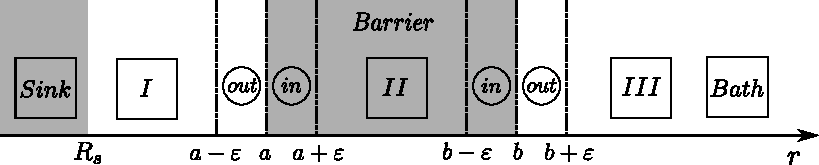
\includegraphics[width = .9 \textwidth]{plots/drawing.pdf}
    \caption{sketch of the spatial discretization for the flow analysis of the system: The Sink and the Barrier are marked in gray. The circles represent narrow volumes of width $\varepsilon$ right at the barrier borders. $\varepsilon$ is set to be one tenth of the barrier width. The squares represent the large spaces between barrier and sink ($I$), between the sink boundaries ($II$) and outside the sink ($III)$. Each volume has the shape of a spherical shell (except the sink which is a sphere). Active and inactive particles are investigated separately in each of these volumes}
    \label{fig:flowchart_scetch}
\end{figure}
For each of these areas one examines the spatial fluxes from and to neighbouring areas and the reactive fluxes from one particle state to the other. \\
For this purpose it is convenient to use the integral form of the continuity equation derived in \eqref{ce0}. To employ it in the actual problem one takes the density profiles to be constant in time such that its left hand side vanishes. Then the terms on the right hand side are calculated separately. The spatial fluxes at the volume boundaries:
\begin{equation}
    J_m^{(S)}(r_i) = \int_{r_i} \vec{j}_m(r) {\rm d} \vec{A}
    \label{spatial_flux}
\end{equation}
and the reactive fluxes from one particle species to the other:
\begin{equation}
    J_{mm'}^{(R)}(r_i,r_j) =\int_{r_i}^{r_j} \left\{ \mathbb{W}_{m'm}\rho_m - \mathbb{W}_{mm'} \rho_{m'} \right\} {\rm d} r
    \label{reaction_flux}
\end{equation}
where $r_i$ and $r_j$. are the radii $R_s$, $a-\varepsilon$, $a$ etc. of the spatial discretization given in figure \ref{fig:flowchart_scetch}.
These fluxes are then represented as arrows between the icons representing the corresponding areas as illustrated in figure \ref{fig:flowchart_scetch}. Active and inactive particles are depicted separately where the icons representing active particles are blue and the icons representing inactive particles are red. \\ \textbf{Interpreting the following flow diagrams it is important to note, that the flows depicted by the arrows are normalized to the largest value for each example. Therefore the arrows only represent \emph{relative importance of fluxes} and have no meaning for their absolute values!} \newpage
. \\ \vspace{-2 cm}

\begin{minipage}[t]{.372 \textwidth}
    \vspace{0.5 cm}
    \begin{figure}[H]
        \caption{Flow diagram for repulsive barrier: This plot shows spatial and reactive particle flows between different particle species (active particles are represented in blue, inactive particles are represented in blue) and different spatial regions (see figure \ref{fig:flowchart_scetch} for reference) for the examples given in figure \ref{rep_symm_dens_profile}. The difference between the different plots is again the decay length which is equal to \newline A): $r_d=250$, B): $r_d=2.5$ and \newline C): $r_d = 0.25$.
    \label{fig:flow_repulsive}}
    \end{figure}
\end{minipage}\hspace{0.02 \textwidth}\begin{minipage}[t]{.608 \textwidth}
    \begin{figure}[H]
        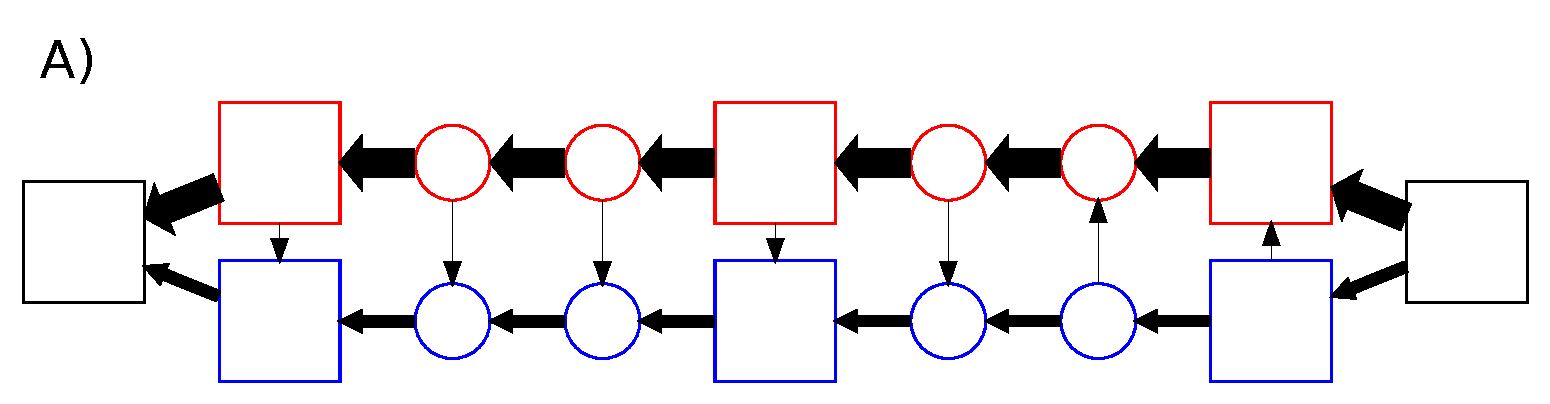
\includegraphics[width = 1 \textwidth]{plots/rep_flowchart0.pdf} 
        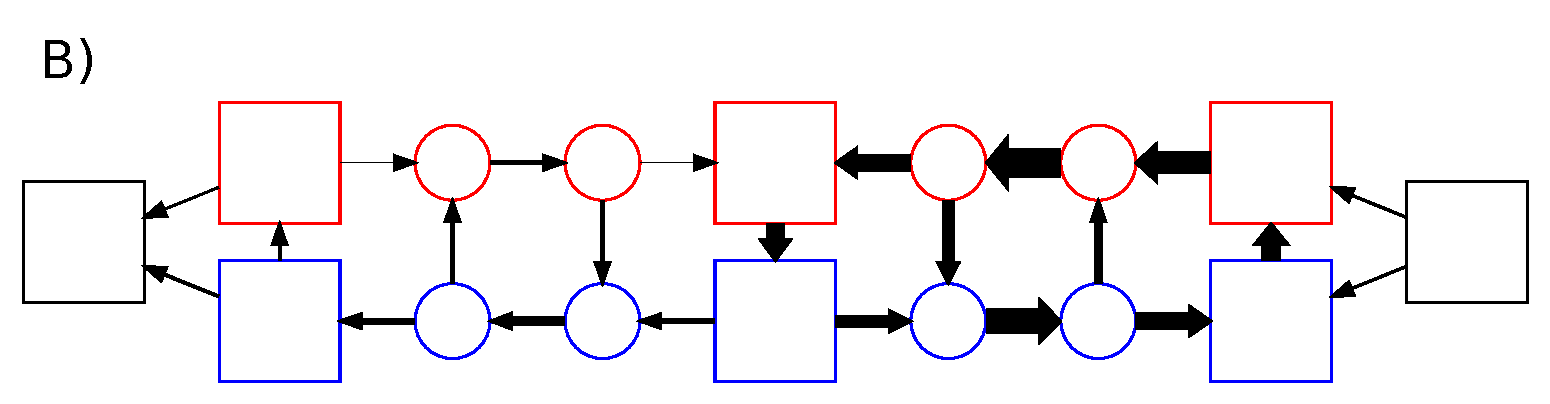
\includegraphics[width = 1 \textwidth]{plots/rep_flowchart1.pdf} 
        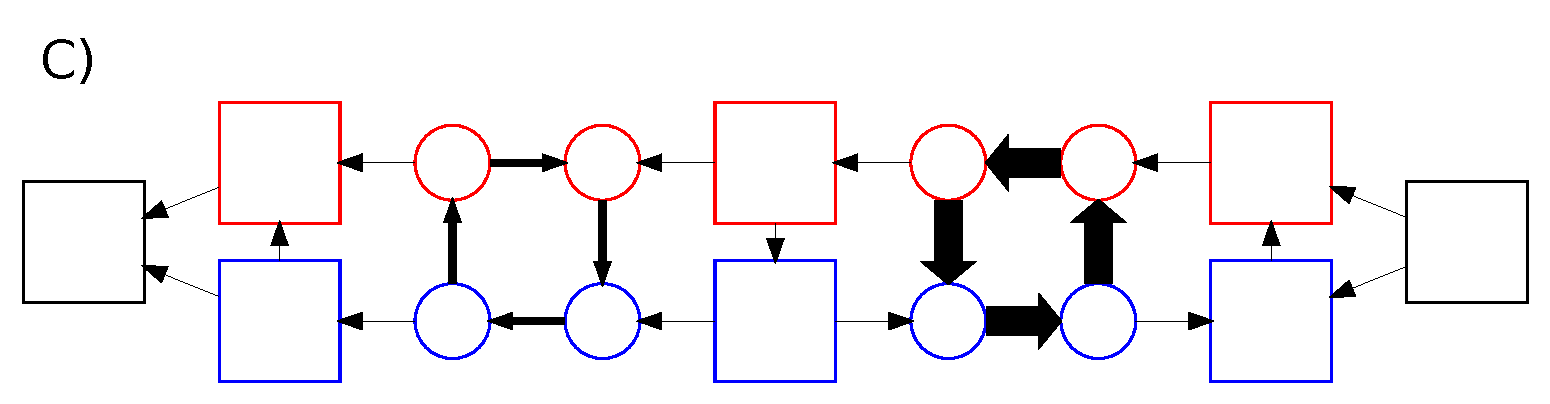
\includegraphics[width = 1 \textwidth]{plots/rep_flowchart2.pdf}
    \end{figure}
\end{minipage}
\vspace{0.5 cm} \\
It is obvious from this illustration that the system behaves qualitatively different depending on its the decay length.
\begin{itemize}
    \item For long decay length as in figure \ref{fig:flow_repulsive} A) it is visible from the very narrow arrows connecting red and blue icons that the particles in both states are independent in good approximation. Therefore inactive particles are not hindered by the barrier on their way from the bath to the sink whereas active particles have to overcome the potential barrier and are thus less likely to interact with the sink. Ether way, particles are very unlikely to change their state in the process. 
    \item For short decay length as in figure \ref{fig:flow_repulsive} C) The behavior is clearly different. Particle movement is closely tied to the potential boundaries at $r=a$ and $r=b$. There active particles are very likely to cross the boundary in downward direction only. Therefore the potential drives a spatial selection of particles that leads to an excess of active particles right outside and a deficit of active particles inside the barrier. The resulting difference in concentration of active and inactive particles at both sides of the barrier boundary leads to a strong reactive fluxes. Inside the barrier particles switch from inactive (red) to active (blue) and outside the barrier they switch from active to inactive state. The resulting imbalance of inactive particles draws them across the barrier from the out to the inside. As obvious from the flow diagram, the result is a strong \emph{circular current}. Since most of the particles switch states before they can diffuse more than $r_d$ away, the process is closely tied to the barrier boundaries. 
    \item For medium decay length as in figure \ref{fig:flow_repulsive} B) These circular currents are still existent but not so closely tied to the boundaries of the barrier. Therefore they they overlap in space. This has the effect that once a particles has crossed the outer boundary of the barrier as part of one circular current it can switch to the other circular current to cross the inner boundary of the barrier. 
\end{itemize}
In the case of an attractive potential barrier the processes at work are quite similar. The differences to the repulsive case are outlined on the basis of the following flow diagrams: \vspace{-.5 cm} \\
\begin{minipage}[t]{.372 \textwidth}
    \vspace{.5 cm}
    \begin{figure}[H]
        \caption{Flow diagram for attractive barrier: This plot shows spatial and reactive particle flows between different particle species (active particles are represented in blue, inactive particles are represented in blue) and different spatial regions (see figure \ref{fig:flowchart_scetch} for reference) for the examples given in figure \ref{att_symm_dens_profile}. The difference between the different plots is again the decay length which is equal to \newline A): $r_d=250$, B): $r_d=2.5$ and \newline C): $r_d = 0.25$.
    \label{fig:flow_attractive}}
    \end{figure}
\end{minipage}\hspace{0.02 \textwidth}\begin{minipage}[t]{.608 \textwidth}
    \begin{figure}[H]
        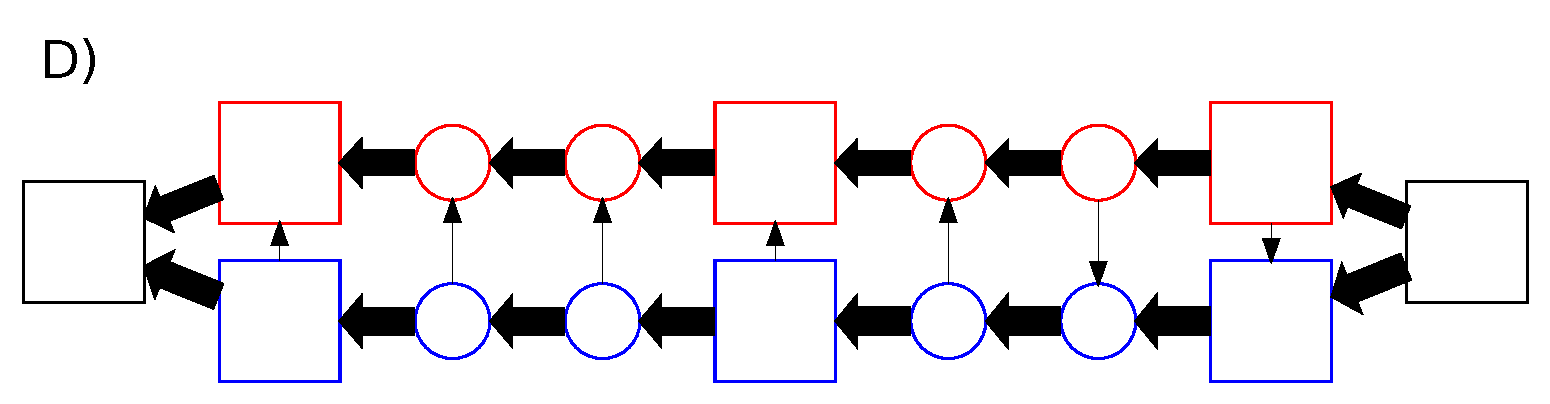
\includegraphics[width = 1 \textwidth]{plots/att_flowchart0.pdf}
        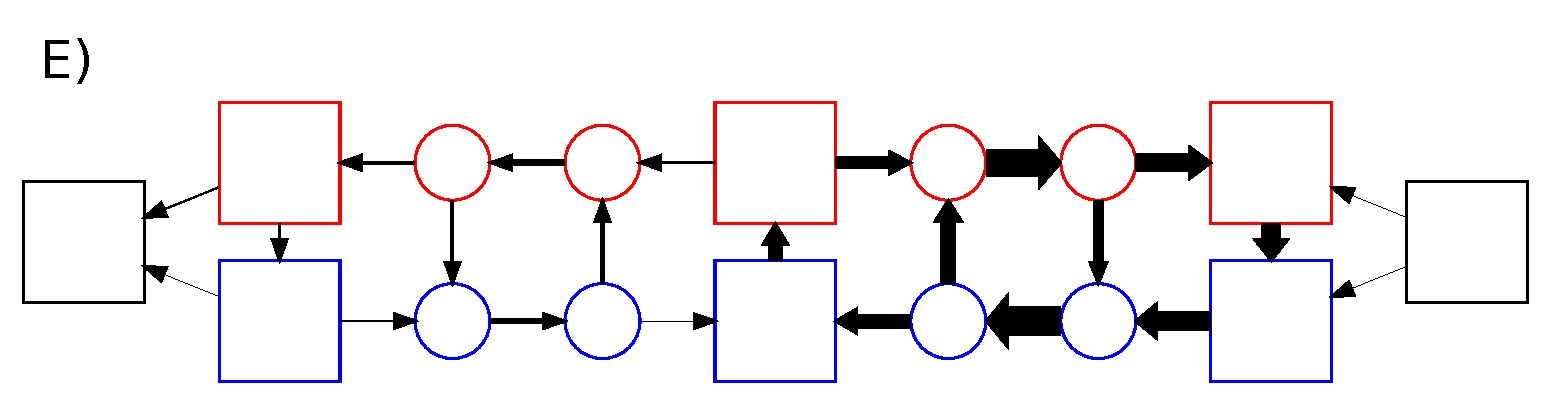
\includegraphics[width = 1 \textwidth]{plots/att_flowchart1.pdf}
        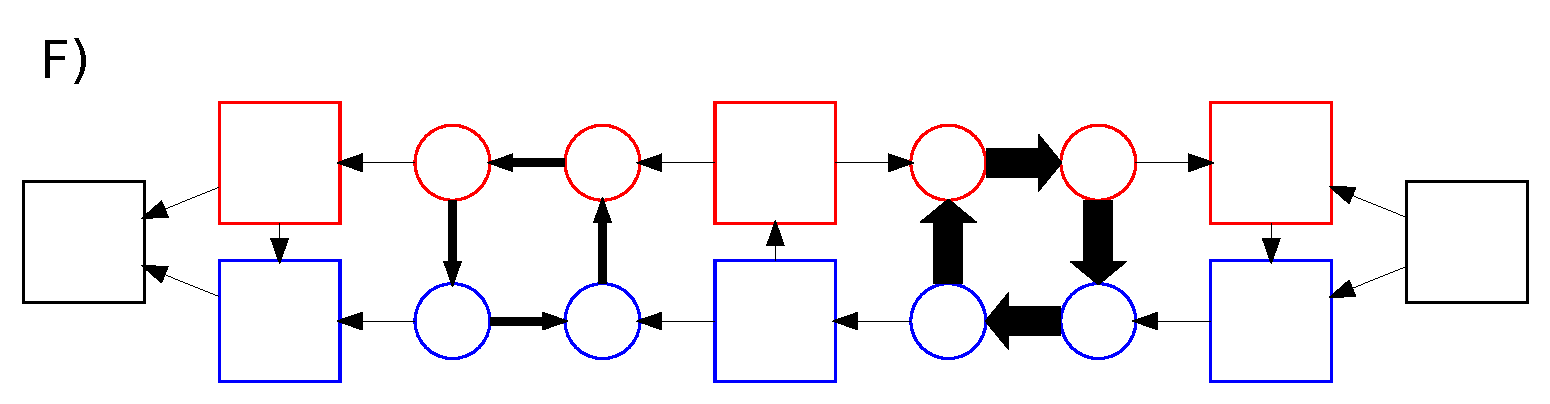
\includegraphics[width = 1 \textwidth]{plots/att_flowchart2.pdf}
    \end{figure}
\end{minipage}
\vspace{.5 cm} \\
The differences to the differences of these examples to the ones presented before in figure \ref{fig:flow_repulsive} can be pointed out one by one:
\begin{itemize}
    \item For long decay length as in figure \ref{fig:flow_attractive} D) the two particle species are independent from each other in good approximation. The difference to the former example is that the active particles are not hindered by the attractive barrier once the steady state is reached. They accumulate in the attractive potential until their concentration is high enough to to make it equally possible for particles to enter and leave the barrier (which es the essentially given by the probability for particles to enter the potential). Therefore both particle species do equally contribute to the flux of particles from the bath to the sink.
    \item For short decay length as in figure \ref{fig:flow_attractive} F) the system again shows strong circular currents around the boundaries of the potential barrier. The difference is here that if active particles now cross the barrier in downward direction this means from the ``out'' to the ``in'' side. Therefore the circular currents are now directed in the other direction (clockwise vs. counter clockwise in this representation)
    \item For medium decay length as in figure \ref{fig:flow_attractive} E)  the two circular currents overlap just as they do in the case of a repulsive barrier. Therefore it is again likely for active particles to be drawn across the outer border of the potential by one current and then cross the boundary of the inner barrier as part of the other current.
\end{itemize}
This analysis has shown how the system behaves qualitatively different depending on switching rate of the barrier or rather depending on the decay length of the particle densities. Knowing this, it is now time to turn to the key quantity in this investigation which is the reaction rate of particles interacting with the sink. 
\subsection{Absorption Rates}
Previously the focus was directed on the distribution of Brownian particles in the system. The distribution was explored for different magnitudes of the systems decay length and qualitative differences were explained by the steady state flow of particles that emerged from the coupling of the barrier fluctuations to the diffusive particle movement.\\
The next section will explore the implication of these qualitative differences on the reaction rate of particles with the sink in the center of the system. This rate can be calculated from the density profiles via equation \eqref{Rate}. In the following the reaction rate is normalized to the Smoluchowski reaction rate $K_S$ \eqref{steady state ideal rate} for an ideal sink without any barrier . This way the influence of the potential barrier can be pointed out explicitly. \\
The decay length $r_d$ is substituted with $1/\alpha$ and the hight of the barrier in units of the thermal energy of the particles $U_2/K_B T$ is substituted by $u$ to maintain a readable form of the results:
\begin{align}
    \frac{K}{K_{S}} &= \frac{F_1}{F_2}
    \label{two_state_rate}
\end{align}
with the nominator $F_1$ and denominator $F_2$ given by the following expressions:
\begin{align*}
    F_1 =& 2 \left(a \left(\alpha-5 b \alpha^2\right)+b \alpha-1\right) e^{2 \alpha (a+b)+u}-2 (a \alpha+1) (b \alpha-1) e^{2 (b+1) \alpha+u}-4 b \alpha (b \alpha+1) e^{3 a \alpha+b \alpha+u} \\
    &+2 b \alpha (b \alpha+1) e^{3 a \alpha+b \alpha+2 u}+4 b \alpha (b \alpha+1) e^{\alpha (a+b+2)+u}-2 b \alpha (b \alpha+1) e^{\alpha (a+b+2)+2 u} \\
    &-2 (a \alpha-1) (b \alpha+1) e^{4 a \alpha+u}+(a \alpha-1) (b \alpha+1) e^{4 a \alpha+2 u}-2 (a \alpha+1) (b \alpha+1) e^{2 (a+1) \alpha+u} \\
    &-(a \alpha+1) (b \alpha+1) e^{2 (b \alpha+u+\alpha)}-(3 a \alpha-1) (b \alpha+1) e^{2 (\alpha (a+b)+u)} \\
    &+(3 a \alpha+1) (b \alpha+1) e^{2 (a \alpha+u+\alpha)}-2 b \alpha (b \alpha+1) e^{\alpha (a+b+2)}+2 b \alpha (b \alpha+1) e^{\alpha (3 a+b)} \\
    &+e^{4 a \alpha} (a \alpha-1) (b \alpha+1)-e^{2 (a+1) \alpha} (a \alpha-1) (b \alpha+1)+(a \alpha+1) e^{2 (b+1) \alpha} (3 b \alpha-1) \\
    &-(a \alpha+1) (3 b \alpha-1) e^{2 \alpha (a+b)} \\
    F_2 =& -4 \alpha \left(a^2 \alpha-a \alpha+a-b \alpha-2\right) e^{\alpha (a+b+2)+u}+2 \alpha \left(a^2 \alpha-a \alpha+a-b \alpha-2\right) e^{\alpha (a+b+2)+2 u} \\
    &-4 \alpha \left(a^2 \alpha-a (\alpha+1)+b \alpha+2\right) e^{3 a \alpha+b \alpha+u}+2 \alpha \left(a^2 \alpha-a (\alpha+1)+b \alpha+2\right) e^{3 a \alpha+b \alpha+2 u} \\
    &+2 \alpha e^{\alpha (a+b+2)} \left(a^2 \alpha-a \alpha+a-b \alpha-2\right)+2 \alpha e^{\alpha (3 a+b)} \left(a^2 \alpha-a (\alpha+1)+b \alpha+2\right) \\
    &-\left(3 \alpha^2 (a (b-2)+2 b)+\alpha (a-3 b+4)-1\right) e^{2 (\alpha (a+b)+u)} \\
    &-2 \left(\alpha^2 (a (5 b+2)-2 b)+\alpha (a+b-4)+1\right) e^{2 \alpha (a+b)+u} \\
    &+2 (a \alpha+1) ((b-2) \alpha+1) e^{2 (b+1) \alpha+u}+2 ((a-2) \alpha-1) (b \alpha+1) e^{2 (a+1) \alpha+u} \\
    &-2 (a \alpha-1) (b \alpha+1) e^{4 a \alpha+u}+(a \alpha-1) (b \alpha+1) e^{4 a \alpha+2 u}+((a+2) \alpha+1) (b \alpha+1) e^{2 (a \alpha+u+\alpha)} \\
    &-(a \alpha+1) ((3 b-2) \alpha+1) e^{2 (b \alpha+u+\alpha)}-e^{2 \alpha (a+b)} \left(\alpha^2 (a (3 b+2)-2 b)+\alpha (-3 a+b+4)-1\right) \\
    &+e^{4 a \alpha} (a \alpha-1) (b \alpha+1)-e^{2 (a+1) \alpha} ((3 a-2) \alpha-1) (b \alpha+1)+(a \alpha+1) e^{2 (b+1) \alpha} ((b+2) \alpha-1)
\end{align*}
Sadly, this form of the solution does not tell very much about the actual behavior of the reaction rate. Nevertheless, it can be used to plot the reaction rate in the case of the two examples that were studied so far: \\
\begin{minipage}[t]{0.5 \textwidth}
    \begin{figure}[H]
        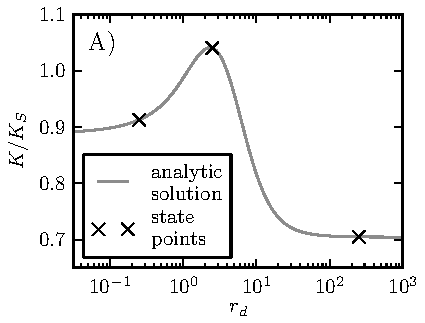
\includegraphics[width = 1 \textwidth]{plots/rb_rate.pdf}
    \end{figure}
\end{minipage}\begin{minipage}[t]{0.5 \textwidth}
    \begin{figure}[H]
        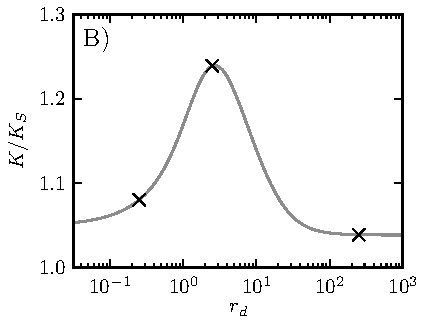
\includegraphics[width = 1 \textwidth]{plots/ab_rate.pdf}
    \end{figure}
\end{minipage}

\begin{minipage}[t]{1 \textwidth}
    \begin{figure}[H]
        \caption{Reaction rate of Brownian particles depending on the decay length of particle density for A) a repulsive barrier and B) an attractive barrier. The decay length and resulting reaction rate for the examples illustrated before are marked with black crosses. Those from figures \ref{rep_symm_dens_profile} and \ref{fig:flow_repulsive}  are marked in A), and Those from figures \ref{att_symm_dens_profile} and \ref{fig:flow_attractive} are marked in B).\label{reaction_rate_examples}}
    \end{figure}
\end{minipage}
\vspace{.5 cm} \\
It is obvious from these plots that the reaction rate converges to finite values for very small and very large decay length and that it takes some maximum value in between. \\
Similar behavior has be studied for escape rates of Brownian particles trapped in fluctuating potentials. In this case the mean first passage time of the trapped particle over the barrier depends on the properties of the potential fluctuations. This has been extensively studied for different barrier shapes and different types of fluctuations \cite{Doering1992, Zurcher1993, Hanggi1994, Pechukas1994,Reimann1995a, Reimann1995}. \\
When Charles Doering and Jonathan Gouda first observed the phenomenon in 1992 \cite{Doering1992} they studied a particle that was trapped between a reflecting wall and a piecewise linear potential barrier that was subject to dichotomous Markovian noise. They observed that the mean first passage time of the particle over the barrier converged to finite values for very small and very long correlation times of the barrier fluctuations and exhibits a minimum in between. For this behavior they coined the term\textbf{ \emph{resonant activation}}.\\
Although this has only been studied for escape problems so far, the results presented here strongly suggest that it is also valid to use the term in the case of reaction rates over fluctuating barriers. \par
Even the underlying processes that have been studied in the previous section section can be identified with those, that were found to be responsible for resonant activation in escape problems.
Referring to a first review paper on the topic published by Peter Reimann and Peter H\"anggi in 1997 \cite{Reimann1997} the case of a repulsive barrier can be identified with what they call ``Type I'' potentials, where particles enter the barrier region when it is in a low state and then get lifted up when the barrier switches to be subsequently able to escape. The case of an attractive barrier can be identified with what they call ``Type II'' or breathing barrier. In this case the part of the barrier that actually fluctuates is located right before the actual boundary that has to be overcome. The particle can enter the fluctuating area while it is in a low state, be then lifted when it changes to a high state and be subsequently able to cross the actual boundary. \par

Now, the next step in studying the vast expression that was derived for the reaction rate \eqref{two_state_rate} is evaluating some limits and trying to make sense of them in a physical way.
\newpage
\subsection{Slow Fluctuation Limit}
For slow fluctuations of the potential barrier the decay length $r_d$ and therefore the spatial influence of the potential barrier becomes large compared to the length scale of the system. \\ 
To evaluate this limit, we use equation \eqref{two_state_fpe} with symmetric rates take the limit of $W \rightarrow 0$ and consider the steady state case.
This results in two independent equations for the two particle species:
\begin{align}
    \frac{\partial \rho_1(r,t)}{\partial t} &= \vec \nabla \left[ D \vec \nabla \rho_1(r,t) \right] \\ \nonumber
    \frac{\partial \rho_2(r,t)}{\partial t} &= \vec \nabla \left[\rho_2(r,t) \vec \nabla \frac{U_2(r)}{\gamma} + D \vec \nabla \rho_2(r,t) \right]
    \label{two_state_fpe_W_to_0}
\end{align}
Where $U_2$ has the form given in \eqref{step_potential}. \\
It is assumed that the detailed balance assumption and therefore the boundary condition for $r \rightarrow \infty$ remains valid despite the formal independence of the particle species.\\
The reaction rates for these independent equations can be calculated using the expressions given in \eqref{steady state ideal rate} and \eqref{K_Debye}. The combined rate can be calculated as the weighted average of the two independent rates. Since the transition rates are taken to be symmetric, this results in:
\begin{align}
    K &= \frac{1}{2} \left[ 4 \pi D R_s^2 + 4 \pi D  \left\{\int_{R_s}^{\infty} \frac{\exp \left[ \frac{U_2(r')}{K_B T}\right]}{r'^2} \rm d r' \right\}^{-1} \right] \\ \nonumber
    &= 2 \pi D \left[ R_s^2 +\left\{\int_{R_s}^{a} \frac{1}{r'^2} \rm d r' + \int_{a}^{b} \frac{\exp \left[ \frac{U_2(r')}{K_B T}\right]}{r'^2} \rm d r' + \int_{b}^{\infty} \frac{1}{r'^2} \rm d r' \right\}^{-1} \right]
\end{align}
Now we evaluate the Integrals and divide by the Smoluchowski reaction rate $K_S = 4 \pi D$. Also $R_s$ is set to one and $U_2/K_B T$ is substituted by $u$:
\begin{align}
    \frac{K}{K_{S}} &= \frac{1}{2} \left[1 + \left\{ 1 -\frac{1}{a} + e^u \left(\frac{1}{a} - \frac{1}{b}  \right) + \frac{1}{b} \right\}^{-1} \right] \nonumber \\
    &= \frac{1}{2}\left[ 1 + \left\{ 1 + \left( \frac{1}{a} - \frac{1}{b} \right)\left( e^u -1 \right) \right\}^{-1} \right] \nonumber \\
    &= \frac{1}{2} \left[ 1 + \left\{ 1 - \frac{(b - a)}{ab}\left(1 - e^u \right) \right\}^{-1} \right] \nonumber \\
    &= \frac{1}{2} \left[ 1 + \frac{ab}{ab - \left( b-a \right)\left(1 - e^u \right)} \right].
    \label{two_state_K_slow}
\end{align}
The result of this somewhat intuitive calculation can now be compared to the slow switching limit of equation \eqref{two_state_rate}.
It proves to be sufficient to do a Taylor expansion around $\alpha_0 = 0$ to obtain
\begin{equation}
    \frac{K}{K_{S}} \approx \frac{(b-a)(1-e^u)-2ab }{2 \left((b-a) \left(1-e^u\right)-ab\right)} + \frac{  (b-a)^2\left(1-e^u\right)^2}{4 \left(ab + (b-a)(1-e^u)\right)^2} \alpha.
    \label{ksa}
\end{equation}
Where the leading therm can be modified to take the form
\begin{equation}
    \lim_{\alpha \rightarrow 0} \frac{K}{K_{S}} =\frac{1}{2}\left(1+ \frac{ab}{ab-(b-a) \left(1-e^u\right)}\right).
    \label{klim0a}
\end{equation}
This is exactly the result, that we obtained by the previous calculation.
\subsection{Fast Fluctuation Limit}
For fast fluctuations of the potential barrier, there is another way to deal with equation \eqref{two_state_fpe}. In the limit of $W \rightarrow \infty$ the diffusion therm can be neglected compared to the reactive therms, such that in the case of symmetric rates $\rho_1(r) \equiv \rho_2(r) = 2\rho(r)$ holds for all $r>R_s$. Therefore both equations can be added resulting in 
\begin{equation}
    2 \frac{\partial \rho(r,t)}{\partial t} = \vec \nabla \left[\rho(r,t) \vec \nabla \frac{U_2(r)}{\gamma} + 2 D \vec \nabla \rho(r,t) \right]
    \label{fast_limit_fpe}
\end{equation} 
In other words this means that the timescale of the switching of particles between different states is much smaller than the timescale of spatial movement of the particles. As a result all particles move subject to a constant potential of mean force that is calculated as the weighted average of the potential in its different states. \\
In the steady state case this again reduces to:
\begin{equation}
    0 = \vec \nabla \left[\rho(r,t) \vec \nabla \frac{U_2(r)}{2\gamma} + D \vec \nabla \rho(r,t) \right]
\end{equation}
such that the steady state rate can be calculated using the Debye formula \eqref{K_Debye}:
\begin{align}
    K &=  4 \pi D \left\{\int_{R_s}^{\infty} \frac{\exp \left[ \frac{U_2(r')}{2 K_B T}\right]}{r'^2} \rm d r' \right\}^{-1} \nonumber \\
    &= 4 \pi D \left\{\int_{R_s}^{a} \frac{1}{r'^2} \rm d r' + \int_{a}^{b} \frac{\exp \left[ \frac{U_2(r')}{2K_B T}\right]}{r'^2} \rm d r' + \int_{b}^{\infty} \frac{1}{r'^2} \rm d r' \right\}^{-1}.
    \label{mean_potential_rate}
\end{align}
The evaluation of the integrals, substitution of $U_2/K_B T$ with $u$ and the normalization by the Smoluchowski reaction rate $K_S$ from equation \eqref{steady state ideal rate} results in:
\begin{equation}
    \lim_{\alpha \rightarrow \infty} \frac{K}{K_S} = \frac{ab}{ab - (b-a)(1-e^{u/2})}.
    \label{K_fast_limit_1}
\end{equation}zugang zu einem thema englisch
Now a useful examination of the fast switching limit of equation \eqref{two_state_rate} requires a bit more work.
To find the behavior in the limit of $r_d \ll 1 $, i.e. $\alpha \gg 1$ one takes a closer look at the different exponents that occur in the numerator and denominator of equation \eqref{two_state_rate}. Namely:
\begin{align}
& e_1 = (3a+b)\alpha, \nonumber \\
& e_2 = (2+2b)\alpha, \nonumber \\
& e_3 = (2+a+b)\alpha, \nonumber \\
& e_4 = 4a\alpha, \nonumber \\
& e_5 = (2+2b)\alpha \quad \textrm{and} \nonumber \\
& e_6 = (2a+2b)\alpha.
\end{align}
Using the fact that $b > a > 1$ we find that for $\alpha \gg 1$ the terms containing $e_6$ will dominate all others. Therefore numerator and denominator can be reduced to
\begin{align*}
    F_1' =& ( 1 + a \alpha + e^u (-1 + 3 a \alpha)) (-1 + 3 b \alpha + e^u (1 + b \alpha))\\
    F_2' =& (-1 + (4 - 3 a + b) \alpha + (2 a - 2 b + 3 a b) \alpha^2 + e^{2 u} (-1 + (4 + a - 3 b) \alpha \\
          &+ 3 (a (-2 + b) + 2 b) \alpha^2) + 2 e^u (1 + (-4 + a + b) \alpha + (2 a - 2 b + 5 a b) \alpha^2)).
\end{align*}
If then again only linear and quadratic terms in $\alpha$ are collected one receives an expression that turns out to be a reasonably good approximation of the fast switching behavior of the solution: 
\begin{align}
    \frac{K}{K_{S}} \approx &a \left(3 e^u+1\right) \left(e^u (b x+1)+3 b x-1\right)-b \left(2 e^u+e^{2 u}-3\right) / \nonumber \\
                          &\left\{a \left(e^{2 u} (3 (b-2) x+1)+2 e^u ((5 b+2) x+1)+3 b x+2 x-3\right) \right.  \nonumber \\
                          & \left. +\left(e^u-1\right) \left(b \left(3 e^u+1\right) (2 x-1)+4 \left(e^u-1\right)\right) \right\}
    \label{kla}
\end{align}
and in the actual limit of $\alpha \rightarrow \infty$ one obtains: 
\begin{equation}
    \lim_{\alpha \rightarrow \infty} \frac{K}{K_{S}} = \frac{a b \left(e^u+3\right)}{ab \left(e^u+3\right)-2(b-a)(1-e^u)}.
    \label{kliminfa}
\end{equation}
This can be simplified to 
\begin{align}
    \lim_{\alpha \rightarrow \infty} \frac{K}{K_S} &= \frac{ab}{ab - (b-a)(1-e^{u/2}) \kappa} \\
    \kappa &= \frac{2(1+e^{u/2})}{e^u + 3}
    \label{K_fast_limit_2}
\end{align}
This is clearly not equal to the limit that was obtained in equation \eqref{K_fast_limit_1}.\par
Now, lets see, if it is possible to understand this difference and to learn something from it. To do so it is useful to properly outline the differences in the derivation of these results.
Therefore it is crucial to realize that it is in fact \emph{two} limits that were taken in the process and that their order differed between the two calculations. One limit is that of the decay length $r_d \rightarrow 0$. The other limit concerns the spatial area of the change of the potential barrier, i.e. the width $r_F$ of the spherical shell in which the Brownian particles are actually subject to a force from the barrier. \\
\vspace{-.8 cm} \\
\begin{minipage}[t]{0.372 \textwidth}
    \begin{figure}[H]
        \caption{Simple sketch to point out the order of limits taken for the derivation of equation \eqref{K_fast_limit_1} and \eqref{K_fast_limit_2}. Both derivations uncouple the original equations to derive an expression for the fast switching limit of the reaction rate but the order of limits differs. \label{sketch_of_limits}}
    \end{figure}
\end{minipage}\hspace{0.01 \textwidth} \begin{minipage}[t]{.608 \textwidth}
\begin{figure}[H]
    \centering
    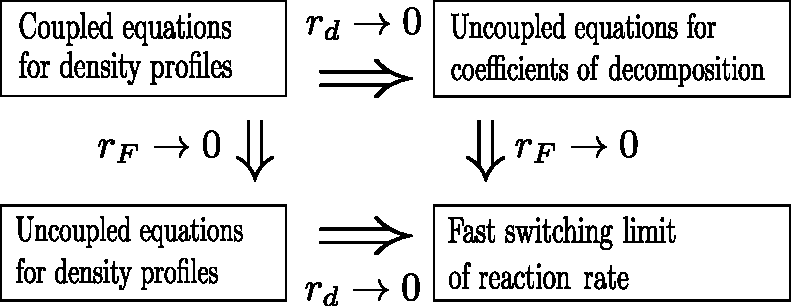
\includegraphics[width = 1 \textwidth]{plots/limits.pdf}
\end{figure}
\end{minipage}\par
Like it is illustrated in figure \ref{sketch_of_limits} the difference is the following: For the derivation of \eqref{K_fast_limit_1} the \emph{first} limit was that of $r_d \rightarrow 0$ and the \emph{second} limit was that of $r_F \rightarrow 0$ whereas for the derivation of \eqref{K_fast_limit_2} the \emph{first} limit was that of $r_F \rightarrow 0$ and the \emph{second} was that of $r_d \rightarrow 0$. \\
Since in general it is not equivalent to take limits in exchanged order it is not unexpected that the resulting expressions differ. The question is now: What does this mean in physical terms? \\

\newpage
\subsection{Numeric study of smooth potential barriers}

The easiest way to get an insight into the final question posed in the last section is to take a closer look at what actually happens, if the potential barrier does not vary in sharp jumps but does so on a finite length scale.
Therefore one examines how the reaction rate depends on the decay length of the particle density given a fixed but finite area on which the barrier changes. The natural way to do this is the application of a potential barrier that resembles a step function in shape and has a parameter to tweak this similarity. A generalized Gaussian:
\begin{equation}
    U_2(r) = U_2 \cdot \exp \left[ - \left( \frac{r_0 - r}{d} \right)^{2n} \right]
    \label{generalized_gaussian}
\end{equation}
with $r_0-d=a$ and $r_0+d=b$ serves this purpose well. The parameter $n$ can be used to control the width $r_F$ of the are of changes in the potential. It decreases as $n$ increases. The reaction rate can then be calculated using the tools described in section \ref{numeric_model}. The results of this procedure are presented in the following figure: \vspace{-0.5 cm}\\

\begin{minipage}[t]{.5 \textwidth}
    \begin{figure}[H]
        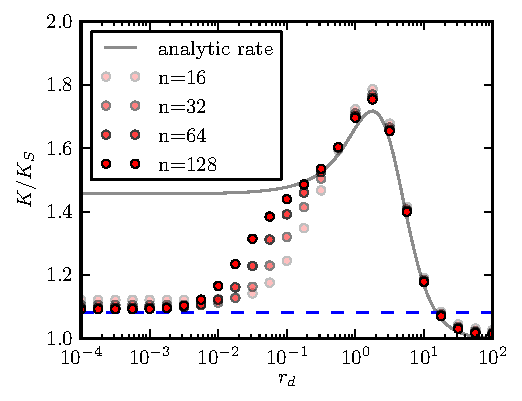
\includegraphics[width = 1 \textwidth]{plots/conv_symmetric.pdf}
    \end{figure}
\end{minipage}\begin{minipage}[t]{.5 \textwidth}
    \begin{figure}[H]
        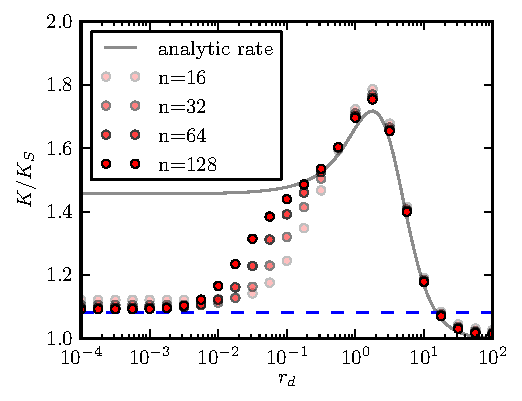
\includegraphics[width = 1 \textwidth]{plots/conv_symmetric.pdf}
    \end{figure}
\end{minipage}

\begin{minipage}[t]{1 \textwidth}
    \begin{figure}[H]
        \caption{Comparison of numeric and analytic results. }
    \end{figure}
\end{minipage}



